\chapter{\normalfont INDEL PHASE ANALYSIS FROM THE SLIDING-WINDOW METHOD}
\label{ch:indel_phase}

\section{Introduction}
Indels refer to insertion and deletion events that can be caused by DNA polymerase errors or incorrect DNA repair during the replication process. The evolutionary history of indels are complicated as their identification, alignments, and annotations \parencite{kunkel2004dna}. Accurate and repetitive methods of identifying indels are necessary for understanding their evolutionary patterns and predicting some gene functions. Especially for indels occurring within the coding domain sequences that have been commonly used as drug targets, protein structure predictors, species diagnostics, and evolutionary markers \parencite{ajawatanawong2013evolution}. \\
\indent Proteins are macromolecules which perform a variety of functions that are essential to organisms, such as catalyzing metabolic reactions, providing structures and support, and transporting molecules within cells and throughout the body \parencite{cozzone2002proteins}. Exons and introns are two features of a gene, where the coding regions are considered as exon parts that are interrupted by non-coding regions known as introns. The coding frames normally begin at the 5’ end with a start codon and stop at the 3’ end with a stop codon \parencite{furuno2003cds}. The function of a coding region can be changed by mutations, including substitutions and indels. A synonymous mutation is a change in the DNA sequences that codes for the same amino acid, while a non-synonymous mutation is a change that codes for different amino acids. Notably, the coding frames must be a continuous stretch of codons in which length is multiple of three. I focus on the indels from the coding regions under selection, while the indels within neutral areas, including intergenic regions and introns, are excluded from our research scope. \\
\indent According to \citeauthor{taylor2004occurrence}, there exists three indel phases in each codon, including phase 0 indels occurring between codons, phase 1 and phase 2 indels occurring from the second and third positions of the codon respectively (Fig 3.1a). Phase 0 indels never change the surrounding amino acids, while phase 1 and phase 2 indels can cause an amino acid substitution that changes the protein sequences. Current codon-aware models can only identify the indels by placing the gap locations between codons without breaking the reading frame. However, they only support the indel events between two adjacent codons and ignore the phase 1 and phase 2 events \parencite{kosiol2007empirical}, which can lead to a misalignment of sequences (Fig 3.1b). \\
\indent Indel-phase analysis are important but understudied components of molecular evolution, which are discussed by a few papers only. \citeauthor{taylor2004occurrence} found an excess of deletions over insertion in rat lineage through a word counting method around all phased-indels symmetrically. \citeauthor{de2007dna} proved that the frequencies of inserted and deleted amino acids differ from background amino acid frequencies in the human proteome by simulating the indel phases and comparing with the observed mammalian data. \citeauthor{hu2013sift} proposed a decision tree algorithm within SIFT to predict the functional effects of amino acids around all indel phases. \citeauthor{zhao2013ddig} developed a support vector machine-based method (DDIG-in) to discriminate between disease-causing and neutral indel phases from the 1,000 Genomes Project. \\
\indent Additionally, insertions and deletions are two different mutational processes.  \citeauthor{kvikstad2007macaque} proposed that insertions are more likely caused by recombination, while deletions are mostly associated with replication-related features. \citeauthor{taylor2004occurrence} found an excess of deletions over insertions particularly for the rat lineage. \citeauthor{lynch2007origins} suggested that there was an overall deletion bias in prokaryotes and insertion bias in most eukaryotes due to the predominance of mobile-element activities. \citeauthor{sjodin2010insertion} found a lower frequency of deletion segregation in humans, providing evidence that deletions were under stronger purifying selection than insertions.\\
\indent In this research, I converted the idea of sliding-window method from previous papers into a computational language (R), and identify all three indel phases. Our method can generate a local optimal alignment by sliding the gaps from each independent window. Unlike current codon-aware aligners that only work with phase 0 indels, this supports all three indel phases. Besides, our results demonstrate that the proportion of three indel phases is strongly correlated with the purifying selection strength in coding regions between focus species and within insertions and deletions separately. Hence, I strongly suggest that including indel phases to generate better alignments, which helps reduce the inflation of estimates of sequence divergence and lead to a more accurate inference of the phylogenetic relationship among species \parencite{kapli2020phylogenetic}. 

\begin{figure}[H]
     \centering
     \begin{minipage}[t]{1\textwidth }
     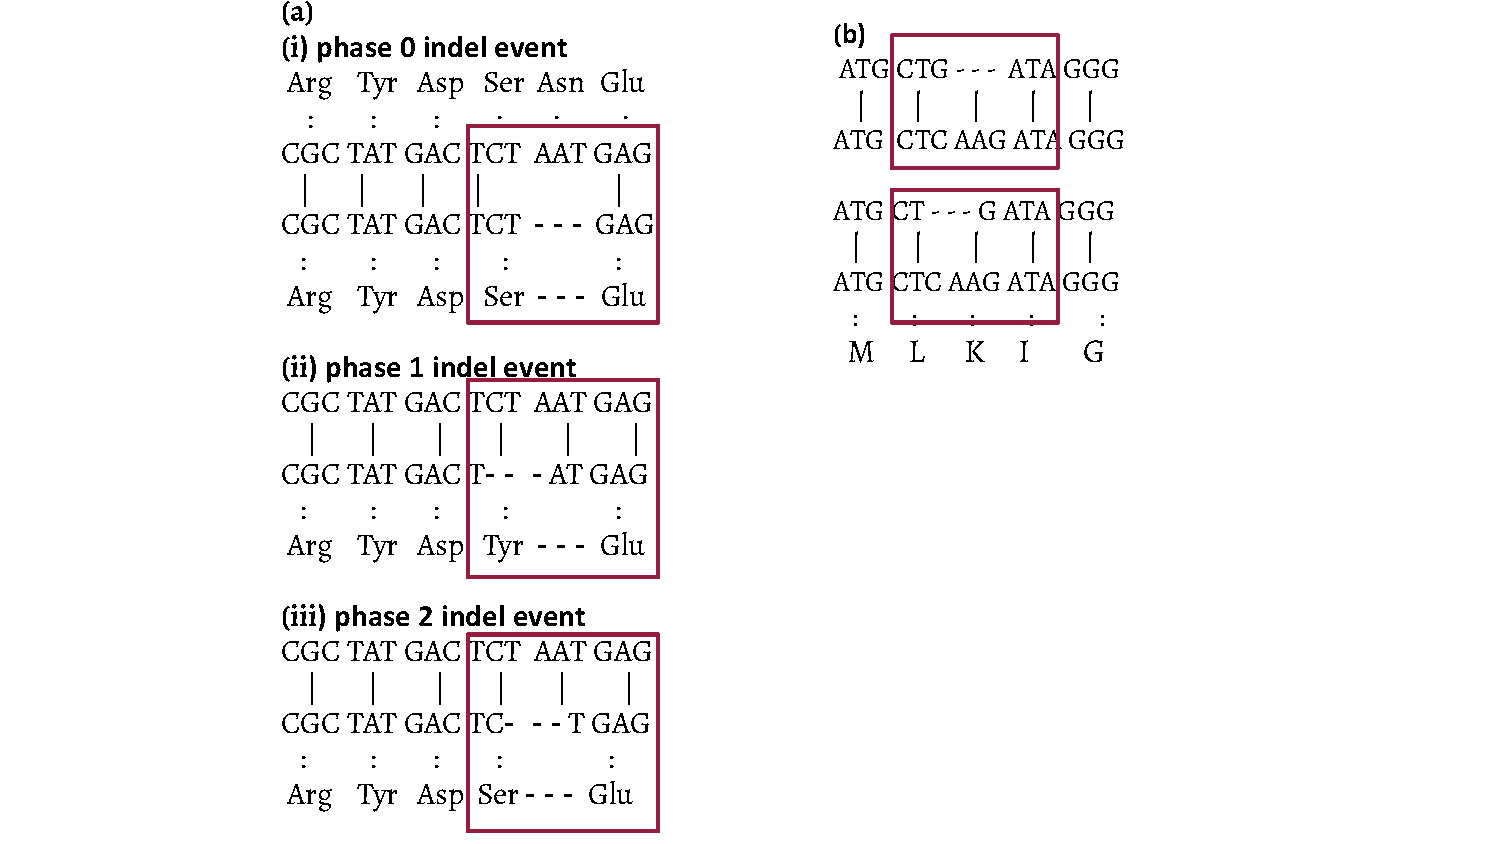
\includegraphics[width=\linewidth]{Fig1.pdf}
     \titlecaption{The Description of Three Different Indel Phases}
     { {a. Phase 0 and phase 2 indel events do not change the adjacent amino acid (Ser, Glu), but phase 1 indel event changes the Ser to Tyr at the left edge of the gap. b. Misalignment due to the limitation of the current codon-aware aligners. (top) phase 0 alignment from the aligner (MAFFT), (bottom) phase 2 alignment from our sw method.}
 \par}
     \end{minipage}
\end{figure}

%%%%%%%%%%%%%%%%%%%%%%%%%%%%%%
\section{Materials \& Methods}
\subsection{Species Choice}
I selected \emph{Mus musculus}, \emph{Rattus norvegicus}, and \emph{Homo sapiens} as my species dataset. The main reasons were twofold: 1) they had a well-annotated genomic region and high-qualified sequence data. 2) They had an appropriate evolutionary branch length. Since a short branch length could cause an insufficient number of indels, and a long branch length might lead to erroneous alignments. Also, I included an outgroup species to help distinguish from insertion to deletion events, through a maximum parsimony method \parencite{saitou1989relative}. 

\subsection{Homology Call}
In order to study the indels between species, I found a series of homologous IDs of genes and transcripts from the Ensembl database. By using the ensembl API (\href{https://rest.ensembl.org/}{https://rest.ensembl.org/}), a set of 14547 homologous genes were extracted. Every gene was identified in each of the human, mouse, and rat (1:1:1 orthologs). Next, I used two main tags (ortholog\_one2one, with\_ccds) to filter out the gene IDs with multiple orthologs and no coding domain sequences (CDS). Then I specified the tag of is\_canonical==1 to extract the canonical transcript from each gene because one gene could have multiple transcripts (Canonical means the longest transcript in Ensembl). And I generated the fasta files of CDS from canonical transcripts. 

\subsection{Sequence Alignment}
I translated all CDS into amino acid using Biostrings::translate in R and specified the parameter of if.fuzzy.codon=solve. Then all fuzzy codons that were translated non ambiguously to an amino acid or stop codon (*) would be translated, and ambiguous fuzzy codons would be translated to X. And I conducted a global alignment of the protein sequences via MAFFT (multiple sequence aligner), since MAFFT was comparatively fast and required no phylogenetic tree beforehand \parencite{katoh2005mafft}. Next, I reversely mapped the alignments back into CDS based on the amino acid to codon ratio (1:3).

\subsection{Quality Control}
Quality control is indispensable in every step of the data extraction process. After downloading the CDS, I filtered out any gene pairs in which the length of sequence were not multiple of three, containing early stop codons, and extra 3' 5' UTR. The last one required the download of a human GTF file (GENCODE) and removed any transcripts with cds\_start\_NF and  cds\_end\_NF tags. Then I measured the alignment similarity of every gene pair in nucleotide and amino acid level between species. The result of the similarity distribution plot (Figure 3.2) demonstrates the high quality of our aligning data, because the similarity score between focal species (mouse and rat) were generally higher than the rest of species pairs, corresponding to the phylogenetic branch length. The file size change of each quality control step can be found in APPENDIX \ref{tab:file_size}. 

\begin{figure}[H]
     \centering
     \begin{minipage}[t]{1\textwidth }
     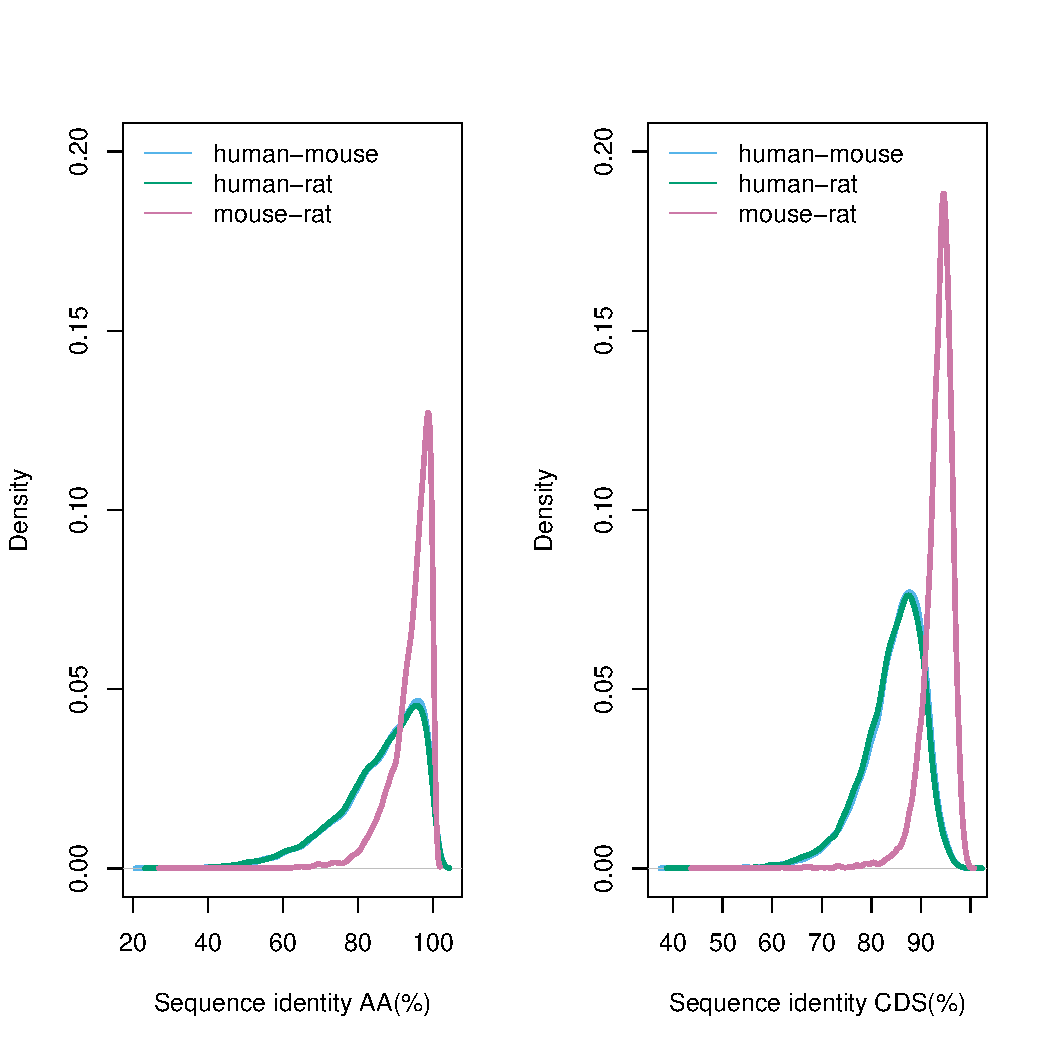
\includegraphics[width=\linewidth]{Fig2.pdf}
     \titlecaption{Similarity Distribution of AA and CDS Sequences in Pairwise Species.}
     {{Left figure represents AA sequence and right figure represents CDS.}
     \par}
     \end{minipage}
\end{figure}

\subsection{Sliding Window Method}
Sliding-window (sw) method was capable of modifying the current alignments by updating the indel phases. The indel length followed a zeta power-law or geometric distribution, and the existence of longer indels was much less frequent in coding sequences \parencite{cartwright2009}. Hence, I only select shorter indels of \{3, 6, 9, 12 nts\} because longer gaps were considered as a combination of short indels together which was unlikely to be influenced by a single evolutionary force (Ex. purifying selection). The sw method treats each gap as a dynamic unit, allowing it to slide from left to right progressively, one nucleotide at a time until reaching out to the edge of the window. The window size was the same as the gap length. After the process of window sliding, 2n alternative alignments would be generated when the window size was n (Fig 3.3a). \\
\indent In order to find the optimal alignment, the similarity score of each alternative alignment was calculated. Figure 3.3a displayed the original (MAFFT) plus alternative alignments of an indel event, among which the highest similarity score was 83.33 $\%$. And if multiple optimal scores appeared, that gap had no single best indel phase and would be marked out as + sign. \\
\indent Moreover, sw method required all of the gap units to be mutually independent and two  rules were created for that purpose: 1) any adjacent gaps of the same sequence cannot be too close to merge into a single gap during the sliding process (Fig 3.3b upper). 2) Any adjacent gaps of different sequences cannot be too close to overlap the same aligning space. (Fig 3.3b lower). All failed gaps were marked out as = sign. 
Additionally, I found that small-sized windows (3 or 6 nt) were supposed to include more gaps due to the extra space generated between each gap unit. Large-sized windows (9 or 12nt) led to a less amount of gaps, while having a higher chance of generating a single optimal alignment due to the extra nucleotides. Hence, making a good choice of the window size was important for the accuracy of the sw method.

\begin{figure}[H]
     \centering
     \begin{minipage}[t]{1\textwidth }
     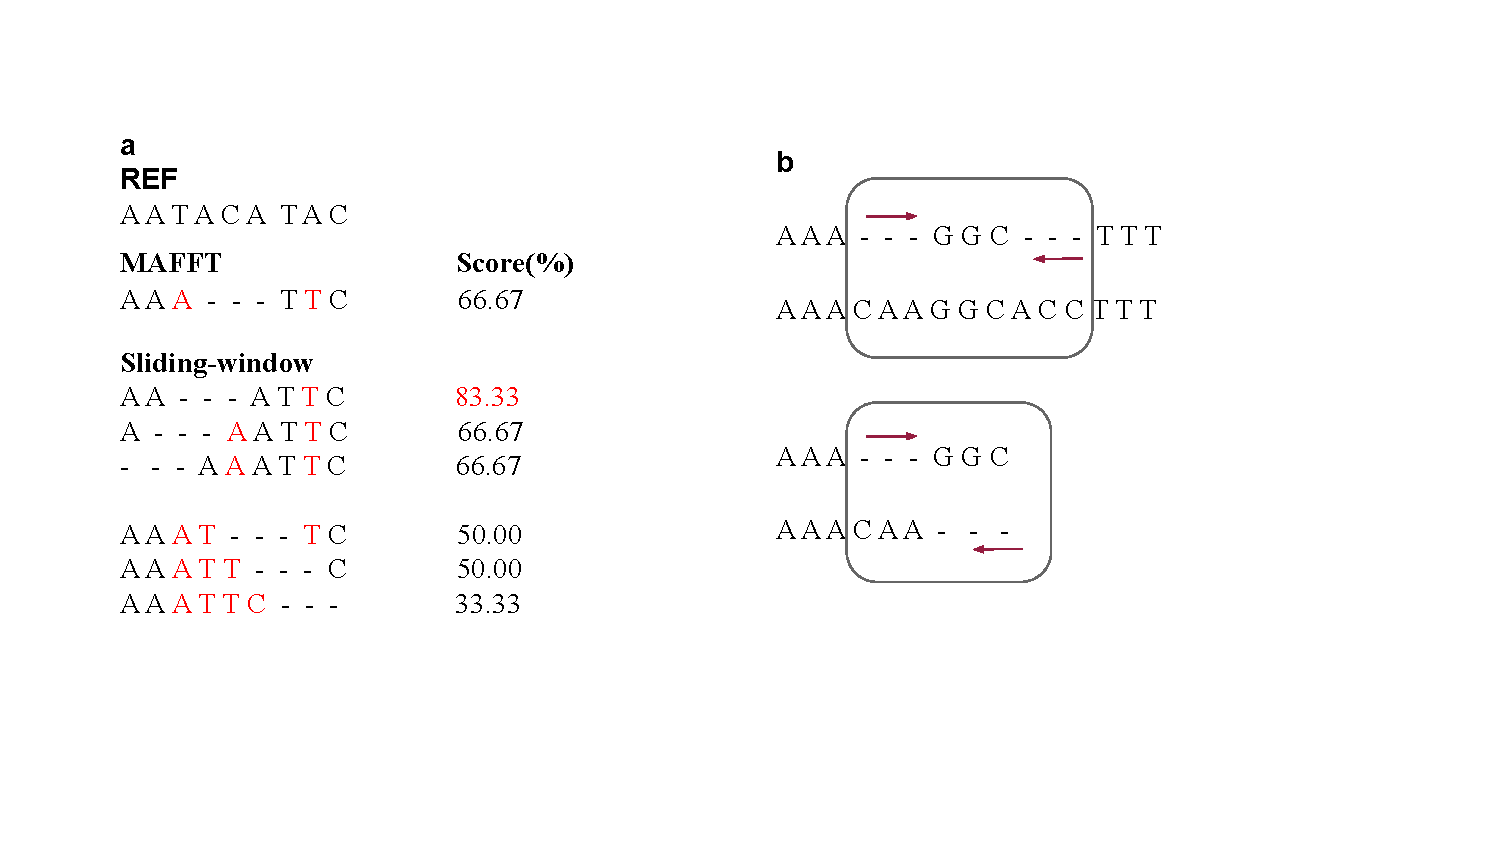
\includegraphics[width=1.2\linewidth]{Fig3.pdf}
     \titlecaption{The Application Rules of Sliding-window Method.}
     {{a. Find an optimal alignment via the sw method. b. Upper alignment is an example of 1st rule violation. Two gaps are very close on the same sequence that can merge into a single gap during the dynamic sliding process. Lower alignment is an example of 2nd rule violation. Two adjacent gaps are on separate sequences that might overlap the same aligning space during the sliding process. (a. arrow -- the moving direction of gaps. b. REF -- reference sequence; MAFFT -- Mafft alignment; sliding-window -- alternative alignments generated by this method, Score -- similarity score based on the percentage of number of matches).} 
 \par}
     \end{minipage}
\end{figure}

\subsection{Identify Three Indel Phases}
All qualified indel events were recorded and distinguished after the sliding window fixation. By taking account of the outgroup species sequence, I was capable of separating from insertions to deletions through the maximum parsimony method. Besides, I calculated the proportion of non-synonymous and synonymous substitutions from phase 1 and phase 2 indels and made a bar plot.  

\subsection{Measure of Power for SW Method}
To test the performance of the sliding window method, I calculated the positional difference of gaps between before and after sw method fixation. The original gap locations were generated by the MAFFT aligner, which was assumed to grab the most true gap locations for its speed and accuracy \parencite{katoh2005mafft}. And I generated a positional difference distribution plot for all gaps, in which the range of distribution is from zero to a defined window size. \\
\indent Furthermore, I investigated the distribution bias by two separate methods: 1) extracting all surrounding codons of each window and summarizing them into 20 distinctive empirical codon model (ECM) subsets based on the codons of similar physico-chemical properties \parencite{kosiol2007empirical}. 2) Reversing the CDS and realigning them using the same method.   

%%%%%%%%%%%%%%%%%%%%%%
\section{Results}
\subsection{Indel Phase Proportions}
Figure 3.4 displays the genome-wide proportion of the indel phases. The upper left histogram shows the indel phase proportion across four different gap lengths in the window size of three nucleotides. Regardless of the window sizes, I find a consistent trend of the proportion of indel phases -- the proportion of phase 0 indels is greater than the proportion of phase 2 indels, greater than the proportion of phase 1 indels.\\
\indent Figure 3.5 displays the proportion of non-synonymous vs synonymous indels from phase 1 and phase 2 events. The proportion of non-synonymous substitutions are much higher in phase 1 indels (about 95\%) than phase 2 indels (about 30\%) across four different window sizes. On the contrary, the proportion of synonymous substitutions are much lower in phase 1 indels (about 5\%) than in phase 2 indels (about 70\%). 

\begin{figure}[H]
     \centering
     \begin{minipage}[t]{1\textwidth }
     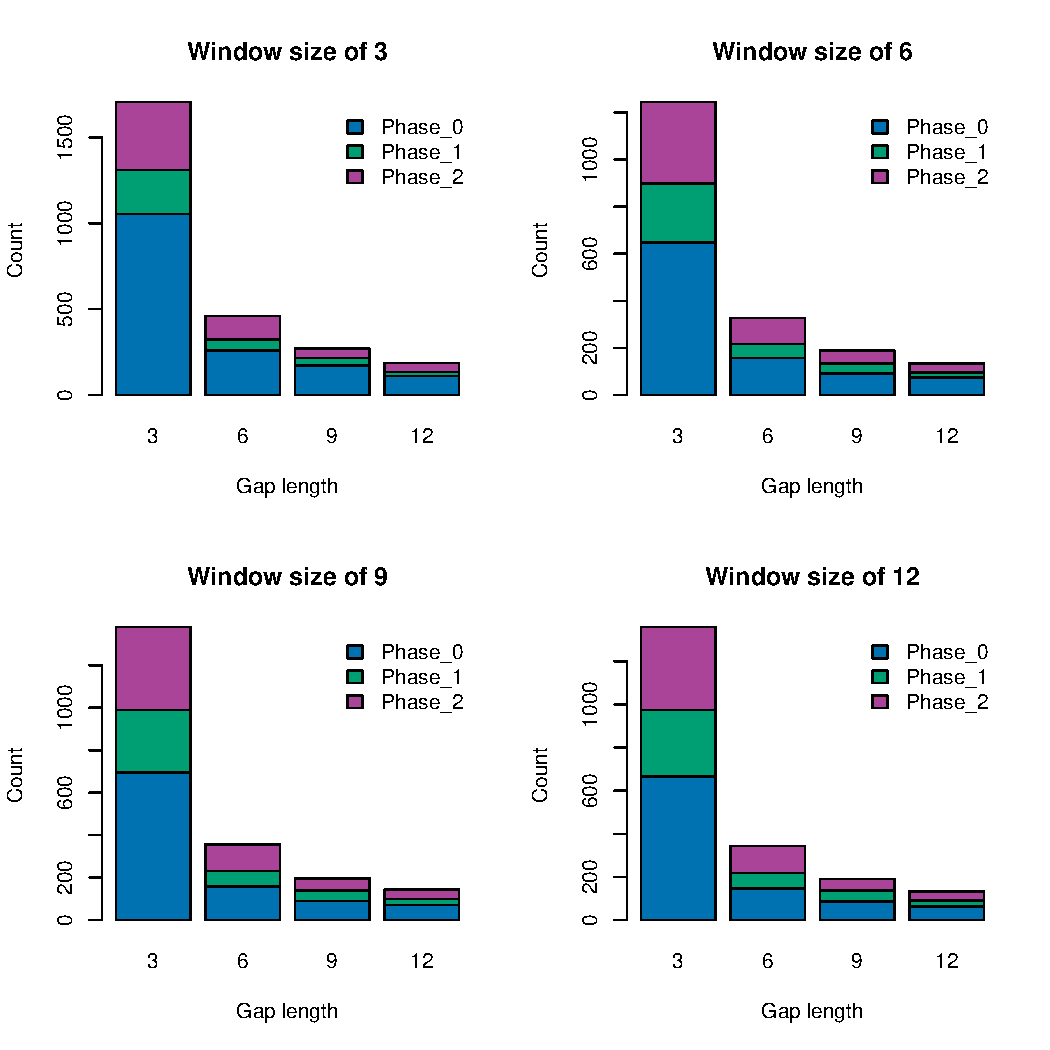
\includegraphics[width=\linewidth, height=\linewidth]{Fig4.pdf}
     \titlecaption{The Proportion of Indel Phases of Different Gap Lengths across Four Window Sizes.}
     { {(X-axis is the gap length, Y-axis is the count of each indel phase).}
 \par}
     \end{minipage}
\end{figure}

\begin{figure}[H]
     \centering
     \begin{minipage}[t]{1\textwidth }
     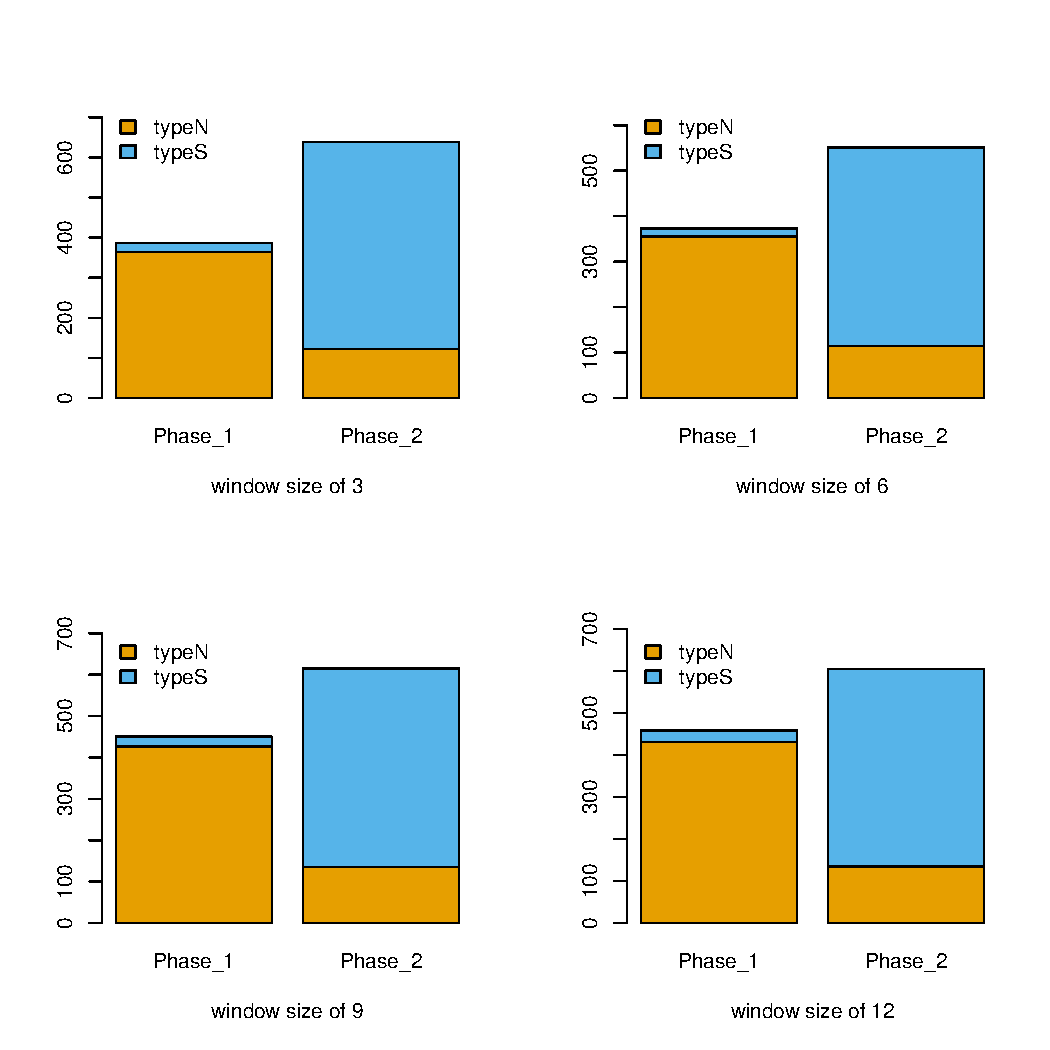
\includegraphics[width=\linewidth, height=\linewidth]{Fig5.pdf}
     \titlecaption{The Proportion of Synonymous vs Non-synonymous Indels within Phase-1 and Phase-2 Events across Four Window Sizes.}
     { {(X-axis is the indel phases, Y-axis is the count of typeN or typeS indels).}\par}
     \end{minipage}
\end{figure}

\indent Figure 3.6 displays the genome-wide proportion of the indel phases of insertion and deletion events separately. Regardless of the window size, there are more deletion events than insertion events within coding regions. Although I find no significant difference of phase proportions between insertion and deletion events, except for phase 1 proportions of window size of 9 and 12, in which their p value of non-parametric chi-squared proportion test are less than 0.05 (APPENDIX \ref{tab:pha_ins_del}). 

\begin{figure}[H]
     \centering
     \begin{minipage}[t]{1\textwidth }
     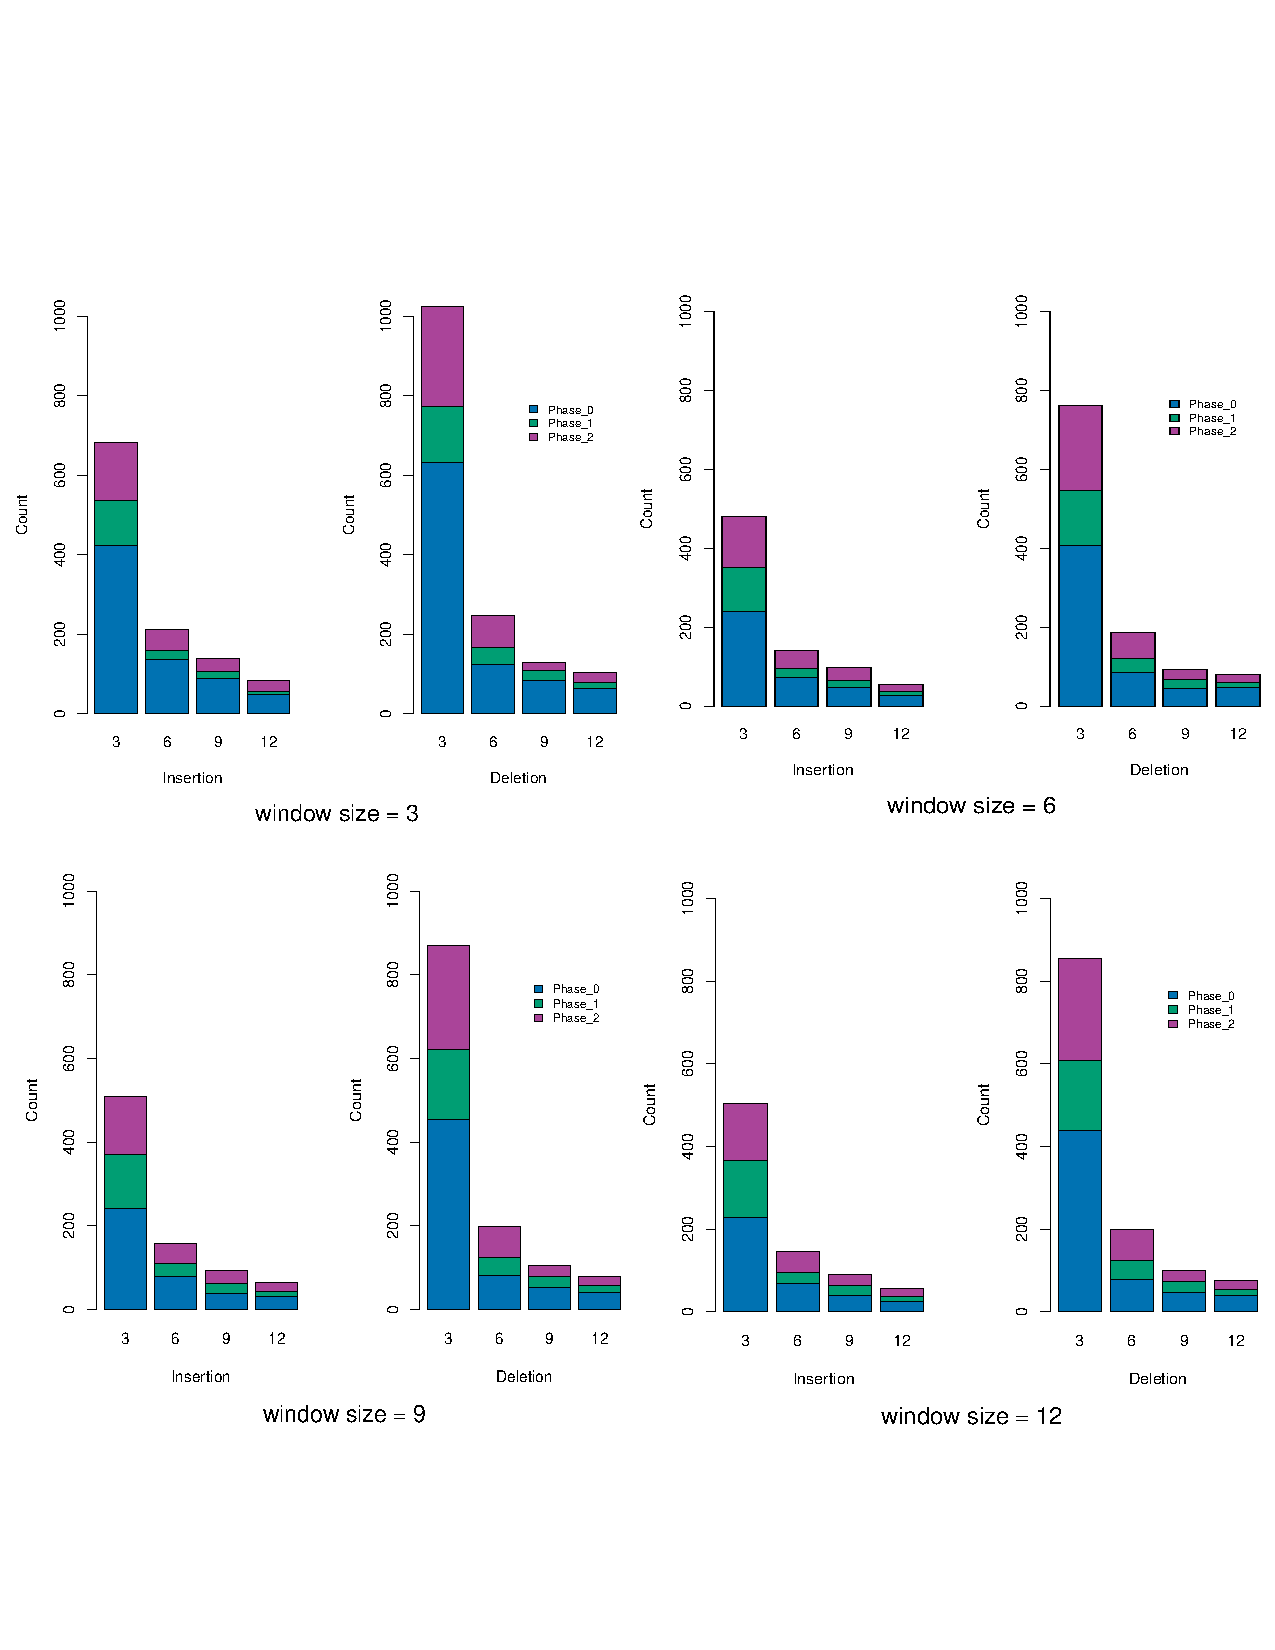
\includegraphics[page=1,width=1\linewidth, height=1.2\linewidth]{Fig6.pdf}
     \titlecaption{The Proportion of Phases of Different Gap Lengths between Insertion and Deletion Events across Four Window Sizes.}
     { {(X-axis is the gap length, Y-axis is the count of each insertion or deletion phase).}\par}
     \end{minipage}
\end{figure}
\newpage

\subsection{Positional Difference of gaps between SW and MAFFT}
Figure 3.7 displays a bell-shaped similar distribution of positional difference of gaps across different window sizes, The frequency density decreases if a gap moves away from its original position zero.  However, this distribution is biased due to the existence of multiple peaks, especially at the right edge of the windows, such as position +3 and +6. I also find that such edge bias is reduced in a larger window size of 9 and 12. \\   
 
\begin{figure}[H]
     \centering
     \begin{minipage}[t]{1\textwidth }
     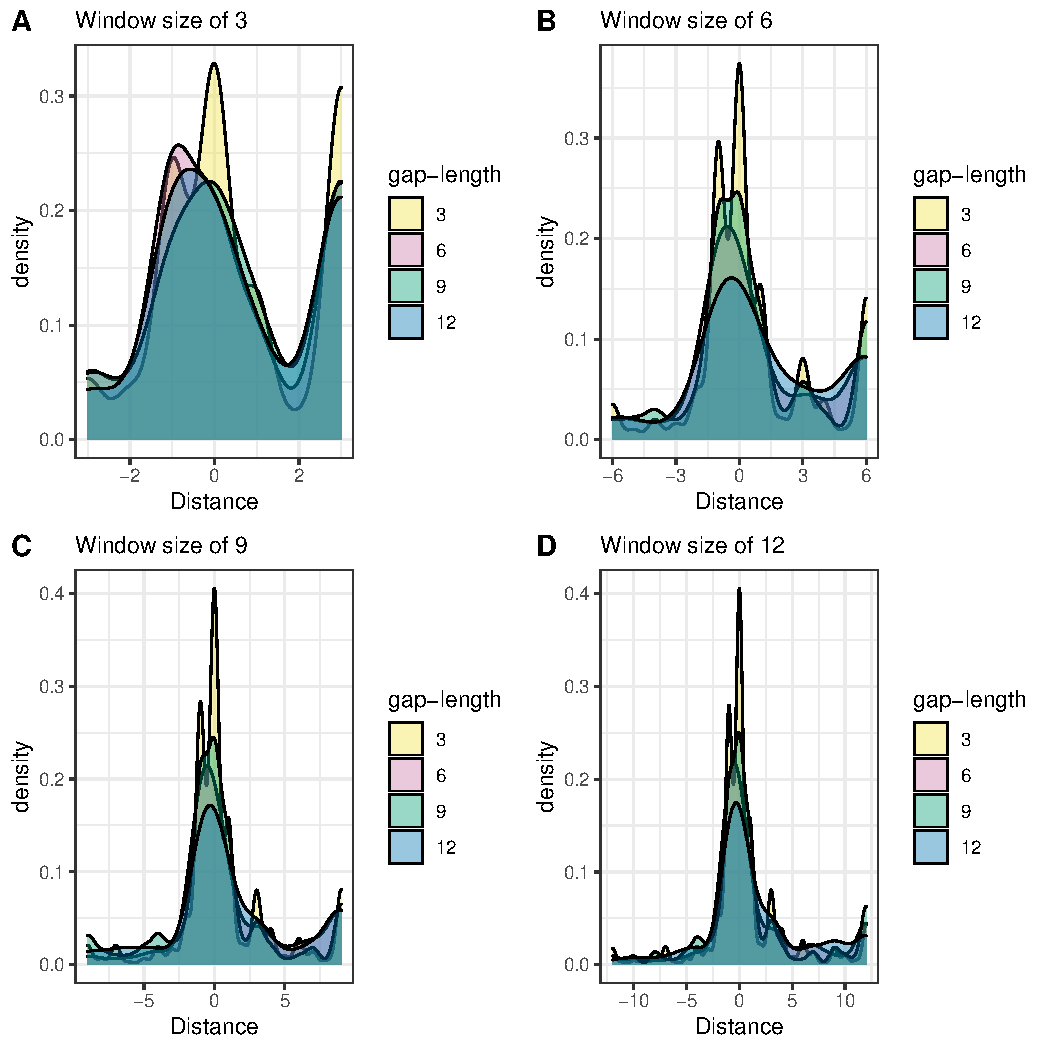
\includegraphics[width=1\linewidth]{Fig7.pdf}
     \titlecaption{Positional Differences of Gap Lengths across Four Window Sizes between the Mafft and SW Method.}
     { {Each position on the x-axis represents the relative nucleotide distance between the original gap position generated by MAFFT and the new position generated by the sw method. All MAFFT gaps are at the position 0 and the sw gaps can be any positions on the x-axis. The y-axis counts the frequencies of each position.}  
 \par}
     \end{minipage}
\end{figure}

%%%%%%%%%%%%%%%%%%%%%%%%%%%%%
\section{Discussion}
\subsection{Indel Phase Analysis}
The proportion of indel phases suggests that the protein coding regions undergo purifying selection in focal species. Since phase 0 indels only change the number of codons, phase 1 and phase 2 indels can change a single surrounding amino acid that encodes. I find that the phase 1 indels are more likely to cause an amino acid substitution due to the less codon degeneracy, indicating that they are the most deleterious events among three. The results from Figure 3.5 also show that the phase 1 indels have a higher chance of resulting in non-synonymous codon substitutions compared with the phase 2 indels. \\ 
\indent Although insertions and deletions are two different processes that are intrigued by distinctive mechanisms, I find a similar trend of phase proportions (phase0$>$phase2$>$phase1) in both.  Although our results provide no evidence that either insertions or deletions are under different selective strength at a significant level, there is an overall deletion bias across four different window sizes within coding regions, which are also published in previous papers. 

\subsection{Positional Difference Distribution Bias}
The probability of finding gaps decreases when the gaps walk away from the original Mafft alignment positions. However, the edge bias from positional difference distribution is asymmetric and multimodal. Here, I propose two hypotheses: 1) In addition to alignment scores, Mafft prefers to place some gaps in a specific position such that the surrounding codons of the similar physico-chemical properties align perfectly. However, this assumption gets rejected because no obvious ECM patterns exist within our aligning windows. 2) Our results from the reversed order alignments displayed more left-edge bias instead of right-edge bias. This suggests that the edge bias is more likely to be a systematic bias within mafft. For example, sequence context might affect the gap position choice in Mafft, especially when there are many repetitive sequence fragments. Additionally, the reduced edge bias in larger window sizes +9, +12 indicates that including more nucleotide information into the windows helps correct the bias. 



 



